
%III 
\section{Mise en place d'un modèle numérique pour le Sled $0,3 g$ \label{ccs_mp_2022_sec_3}}

\ifprof
\else
Le bureau d'études décide de poursuivre le dimensionnement en modélisant l'asservissement du Sled. Il sera ainsi possible de définir la structure de commande de l'actionneur qui permettra de respecter les exigences définies dans le diagramme présenté en figure \ref{ccs_mp_2022_fig_A}.
\fi

%III.A -
\subsection{Commande en vitesse sans correction \label{ccs_mp_2022_sec_3A}}
\begin{obj}
L'objectif consiste dans un premier temps à valider, à partir d'un modèle, le principe d'une structure d'asservissement en vitesse, sur une commande en accélération.
\end{obj}

\ifprof
\else
Un premier modèle multiphysique (modèle $\mathrm{n}^{\circ} 1$, figure \ref{ccs_mp_2022_fig_20}) a été réalisé par les ingénieurs du bureau d'études à partir des éléments fournis par le prédimensionnement réalisé précédemment.

\subsubsection*{Hypothèses d'étude}
Le modèle proposé comporte trois parties :
\begin{itemize}
  \item une partie électrique avec un moteur contrôlé en courant qui convertit l'énergie électrique en énergie mécanique en rotation ;
  \item une partie mécanique en rotation constituée d'un axe moteur et de ses frottements internes ;
  \item une partie mécanique en translation issue d'un dispositif de transformation de mouvement de rotation en mouvement de translation. Le dispositif associé de type pignon-crémaillère est considéré parfaitement rigide. Cette partie mécanique en translation comporte les différentes masses embarquées : plateforme + siège + capteurs et volontaire.
\end{itemize}

La particularité de ce modèle réside dans le fait qu'il s'agit d'une structure d'asservissement en vitesse, sur une commande en accélération. En effet, afin de répondre à la problématique exposée en introduction, la consigne appliquée au modèle est une accélération de $+0,3 g$ appliquée pendant une durée de 1 seconde, suivi d'une accélération de $-0,3 g$ (ou décélération) appliquée pendant une durée de 1 seconde également (figure \ref{ccs_mp_2022_fig_04}).

Les performances attendues (stabilité, précision, rapidité...) et définies dans le diagramme des exigences (figure \ref{ccs_mp_2022_fig_A}) sont donc des performances en accélération (sauf indication contraire). Cette consigne en accélération est adaptée pour permettre la commande en vitesse du moteur. Un asservissement en vitesse est réalisé à l'aide d'un capteur de vitesse de gain unitaire.
\fi

%Q 13. 
\question{\label{ccs_mp_2022_sec_q_13}Quels sont les rôles respectifs des blocs A et B du modèle $\mathrm{n}^{\circ} 1$ (figure \ref{ccs_mp_2022_fig_20}) ?}
\ifprof
\begin{corrige}
Le bloc A est un intégrateur : $A(p) = \dfrac{1}{p}$.
Le bloc B est un dérivateur : $B(p) = p$.
\end{corrige}
\else
\fi

\ifprof
\else
La modélisation multiphysique proposée peut ainsi être modélisée sous la forme d'un schéma bloc (figure \ref{ccs_mp_2022_fig_07}).

\begin{figure}[!h]
\centering
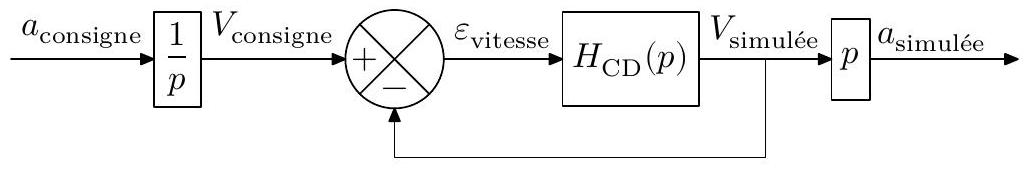
\includegraphics[width=.7\textwidth]{2025_07_06_ec63d2f3afc18cdeeb83g-05}
%Figure 7
\caption{\label{ccs_mp_2022_fig_07}Modélisation $\mathrm{n}^{\circ} 1$ du Sled sous forme de schéma bloc à retour unitaire}
\end{figure}




\subsubsection*{Notations et données}
\begin{itemize}
  \item L'ensemble des trois parties du modèle décrites précédemment (électrique, mécanique en rotation et mécanique en translation) constitue la chaine directe du système que l'on modélise par la fonction de transfert $H_{\mathrm{CD}}(p)$.
  \item La fonction de transfert de l'asservissement en accélération est modélisée sous la forme
\end{itemize}

$$
H_{\mathrm{acc}}(p)=\frac{\text { Accélération simulée }(p)}{\text { Consigne accélération }(p)}=\frac{a_{\text {simulée }}(p)}{a_{\text {consigne }}(p)} .
$$

\begin{itemize}
  \item La fonction de transfert de l'asservissement en vitesse en boucle ouverte peut s'écrire sous la forme d'un second ordre :
\end{itemize}

$$
H_{\mathrm{BO}}(p)=H_{\mathrm{CD}}(p)=\frac{\text{Vitesse simulee}(p)}{\text{Ecart vitesse}(p)}=\frac{V_{\text {simulée }}(p)}{\varepsilon_{\text {vitesse }}(p)}=\frac{K_{\mathrm{BO}}}{1+\frac{2 \xi_{\mathrm{BO}}}{\omega_{0_{\mathrm{BO}}}} p+\frac{1}{\omega_{0_{\mathrm{BO}}}^{2}} p^{2}} .
$$

\begin{itemize}
  \item La fonction de transfert de l'asservissement en vitesse en boucle fermée est modélisée sous la forme :
\end{itemize}

$$
H_{\mathrm{BF}}(p)=\frac{\text { Vitesse simulée }(p)}{\text { Consigne vitesse }(p)}=\frac{V_{\text {simulée }}(p)}{V_{\text {consigne }}(p)} .
$$

\begin{itemize}
  \item Il est rappelé que pour la pulsation de résonance, notée $\omega_{r}$, le gain en décibel s'exprime sous la forme :
\end{itemize}

$$
G_{\mathrm{dB}-\mathrm{BO}}\left(\omega=\omega_{r}\right)=20 \log \left(\frac{K_{\mathrm{BO}}}{2 \xi_{\mathrm{BO}} \sqrt{1-\xi_{\mathrm{BO}}^{2}}}\right)
$$

Pour effectuer la commande en accélération du modèle $\mathrm{n}^{\circ} 1$ (figure \ref{ccs_mp_2022_fig_20}), les ingénieurs du bureau d'études proposent de travailler sur la commande en vitesse.
\fi

%Q 14. 
\question{\label{ccs_mp_2022_sec_q_14}Justifier cette proposition en déterminant la fonction de transfert en accélération $H_{\text {acc }}(p)$ en fonction de $H_{\mathrm{BF}}(p)$. Conclure sur l'intérêt de cette proposition.}
\ifprof
\begin{corrige}
$$H_\text{acc}(p) = \dfrac{1}{{p}} \times H_\text{BF}(p) \times {p} = H_\text{BF}(p)$$

L'intérêt de cette proposition est de pouvoir contrôler le système en vitesse, à l'aide d'une mesure d'accélération (plus simple à implémenter sur le système à l'aide d'un accéléromètre qui fournit directement l'accélération du solide $S$.
\end{corrige}
\else
\fi

\ifprof
\else
Une première simulation avec ce modèle $\mathrm{n}^{\circ} 1$ (figure \ref{ccs_mp_2022_fig_20}) permet d'obtenir le diagramme de Bode de l'asservissement en vitesse en boucle ouverte $H_{\mathrm{BO}}(p)$, proposé en figure \ref{ccs_mp_2022_fig_08} .

\begin{figure}[!h]
\centering
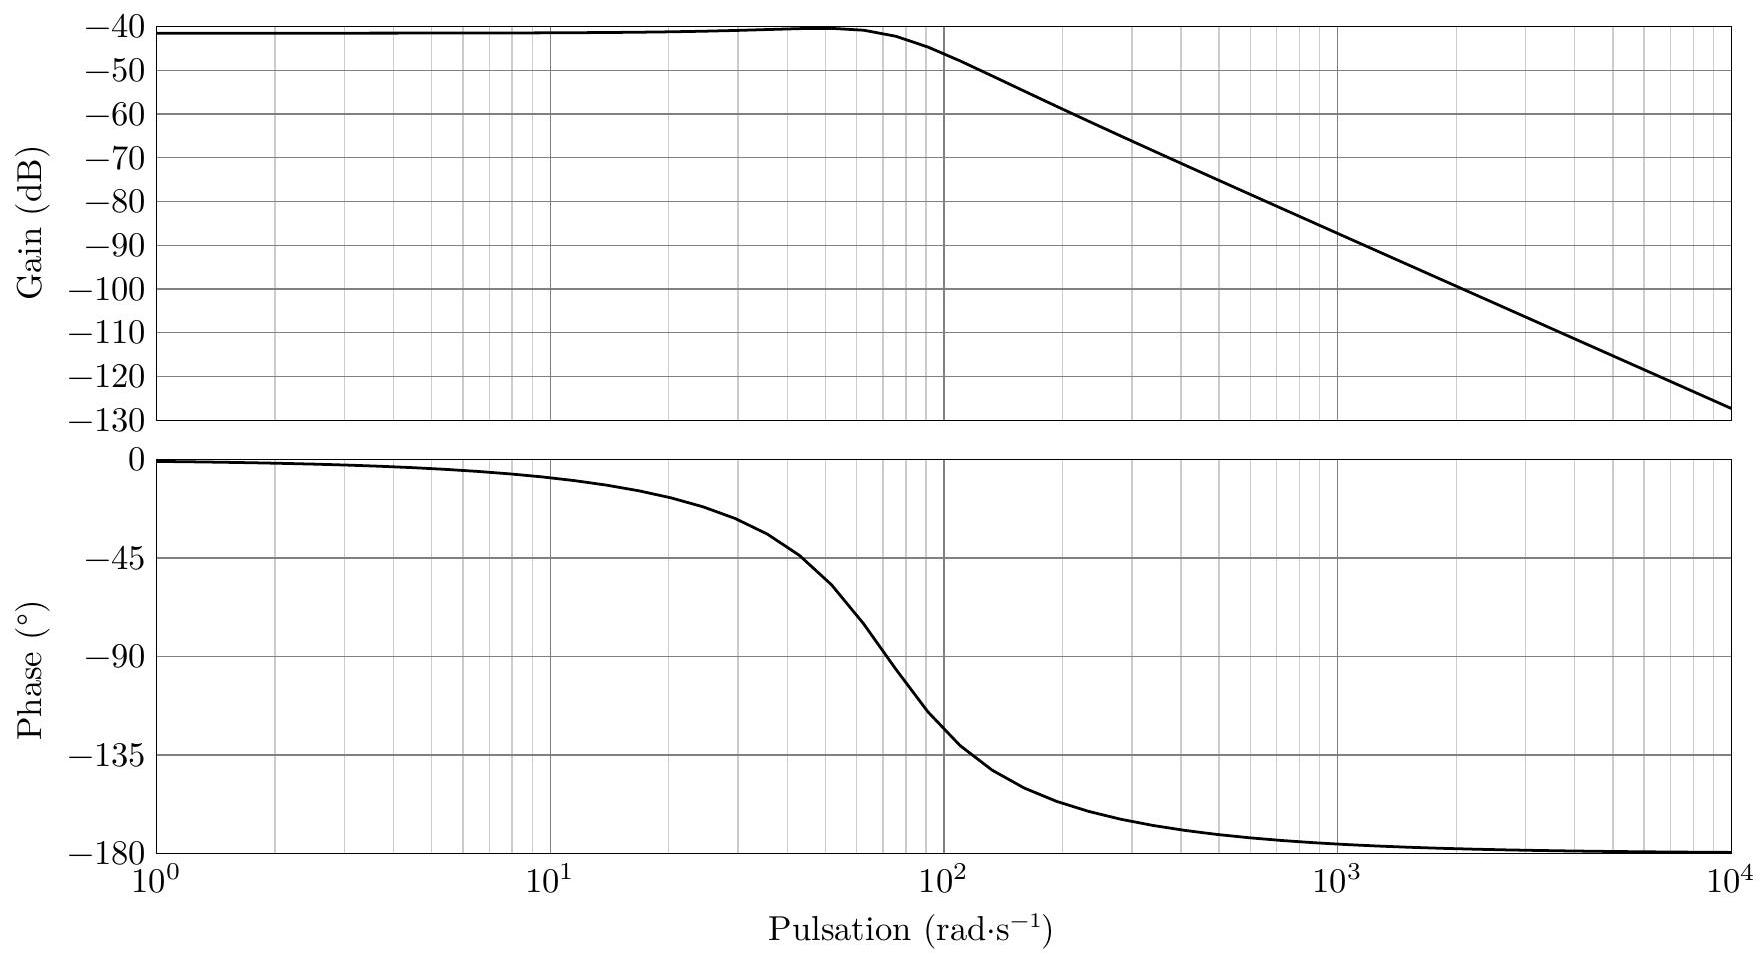
\includegraphics[width=\textwidth]{2025_07_06_ec63d2f3afc18cdeeb83g-06}
%Figure 8 
\caption{\label{ccs_mp_2022_fig_08}Diagramme de Bode en boucle ouverte de l'asservissement en vitesse du modèle $\mathrm{n}^{\circ} 1$ (figure \ref{ccs_mp_2022_fig_20})}
\end{figure}
\fi


%Q 15. 
\question{\label{ccs_mp_2022_sec_q_15}Évaluer graphiquement les marges de stabilité du système et conclure sur le respect de l'exigence Id =1.1.1.1.1.}
\ifprof
\begin{corrige}
L'exigence \texttt{Id = 1.1.1.1.1} requiert une marge de gain $M_\text{gain} > 7$ dB et une marge de phase $M_\varphi > 30$°.

En \textsc{Figure} \ref{fig:sled8}, on remarque que le gain n'est jamais positif ou nul, la marge de phase est donc infinie (ou n'existe pas). De même, la phase n'atteint jamais la valeur de $-180$°, on peut observer une asymptote, la marge de gain est donc infinie (ou n'existe pas).

L'exigence \texttt{Id = 1.1.1.1.1} est donc respectée. 
\end{corrige}
\else
\fi


Une résonance de $+1,1 \mathrm{~dB}$ par rapport à l'asymptote horizontale située à $-41,5 \mathrm{~dB}$ est observée à la pulsation de $49,4 \mathrm{rad} \cdot \mathrm{s}^{-1}$.

%Q 16. 
\question{\label{ccs_mp_2022_sec_q_16}Calculer les valeurs numériques des paramètres $K_{\mathrm{BO}}, \omega_{0_{\mathrm{BO}}}$ et $\xi_{\mathrm{BO}}$ de la fonction de transfert en boucle ouverte $H_{\mathrm{BO}}(p)$ de l'asservissement en vitesse.}
\ifprof
\begin{corrige}
\begin{description}
\item[$K_\text{BO}$] : si l'asymptote horizontale est située à $-41.5$ dB, alors on a
$$ 20\text{log}_{10} (K_\text{BO}) = -41.5 \Leftrightarrow K_\text{BO} = 10^{-41.5/20} = 8.41 \times 10^{-3}$$

\item[$\xi_\text{BO}$] : le gain en décibel lors de la pulsation de résonance permet de déterminer la valeur du facteur d'amortissement. On a $20 \text{log}_{10} \left( \left| H_\text{BO}(j \omega_\text{reson.}) \right| \right)= 20 \text{log}_{10} \left( \dfrac{K_\text{BO}}{\sqrt{\left(  1 - \left( \dfrac{\omega_\text{reson.}}{\omega_{0_\text{BO}}} \right)^2\right)^2 +  \left(\dfrac{2 \xi_\text{BO} \omega_\text{reson.}}{\omega_{0_\text{BO}}}\right)^2} }\right)$

d'après la relation de la pulsation de résonance $\omega_\text{reson.} = \omega_{0_{BO}} \times \sqrt{1 - 2 \xi_\text{BO}^2}$, on obtient le gain en décibel suivant :

$\begin{array}{ll}
20 \text{log}_{10} \left( \left| H_\text{BO}(j \omega_\text{reson.}) \right| \right) &= 20 \text{log}_{10} \left( \dfrac{K_\text{BO}}{\sqrt{\left(  1 - \sqrt{1 - 2 \xi_\text{BO}^2}\right)^2 +  \left(2 \xi_\text{BO} \sqrt{1 - 2 \xi_\text{BO}^2}\right)^2} }\right)\\
 & = 20 \text{log}_{10} (K_\text{BO}) - 20 \text{log}_{10}\left( 2\xi_\text{BO} \sqrt{1 - \xi_\text{BO}^2}\right)\\
\end{array}
$

d'où :

\begin{minipage}{.35\textwidth}
\def\arraystretch{2}
$\begin{array}{ll}
&- 20 \text{log}_{10}\left( 2\xi_\text{BO} \sqrt{1 - \xi_\text{BO}^2}\right) = 1.1\\
\Leftrightarrow & 2 \xi_\text{BO} \sqrt{1 - \xi_\text{BO}^2} = 10^{-1.1/20}\\
\Leftrightarrow & 4 \xi_\text{BO}^2 \left(1 - \xi_\text{BO}^2\right) = 10^{-2.2/20}\\
\Leftrightarrow & 4 \xi_\text{BO}^2 - 4 \xi_\text{BO}^4 = 10^{-2.2/20}\\
\Leftrightarrow & 4 \xi_\text{BO}^4 - 4 \xi_\text{BO}^2 + 10^{-2.2/20} = 0\\
%\Leftrightarrow & 4 \xi_\text{BO}^2 - 4 \xi_\text{BO}^4 = 10^{-2.2/20}\\
\end{array}
$
\end{minipage}
\begin{minipage}{.65\textwidth}
\def\arraystretch{2}
$\begin{array}{l}
\Delta = (-4)^2 - 4 \times 4 \times 10^{-2.2/20} \simeq 3.6\\
\xi_\text{BO}^2 = \dfrac{-(-4)\pm\sqrt{\Delta}}{2 \times 4} = \{0.737; 0.263\} \\
\xi_\text{BO} = \{0.859; 0.513\}  \text{\quad (car $\xi_\text{BO}$ est défini positivement)}\\
\xi_\text{BO} = 0.513  \text{\quad (car la résonance impose $\xi_\text{BO} < \sqrt{2}/2 \simeq 0.707$)}
\end{array}
$
\end{minipage}


\item[$\omega_{0_\text{BO}}$] : on a simplement $ \omega_{0_\text{BO}} = \dfrac{\omega_\text{reson.}}{\sqrt{1 - 2 \xi_\text{BO}^2}}$
A.N. :
$ \omega_{0_\text{BO}} = \dfrac{49.4}{\displaystyle\sqrt{1 - 2 \times 0.513^2}} \simeq 71.8 \text{ rad.s}^{-1}$.
\end{description}
\end{corrige}
\else
\fi


%Q 17. 
\question{\label{ccs_mp_2022_sec_q_17}Déterminer la fonction de transfert en boucle fermée $H_{\mathrm{BF}}(p)$ en fonction de $K_{\mathrm{BO}}, \omega_{0_{\mathrm{BO}}}$ et $\xi_{\mathrm{BO}}$. Identifier ses coefficients $K_{\mathrm{BF}}, \omega_{0_{\mathrm{BF}}}$ et $\xi_{\mathrm{BF}}$ en fonction de $K_{\mathrm{BO}}, \omega_{0_{\mathrm{BO}}}$ et $\xi_{\mathrm{BO}}$.}
\ifprof
\begin{corrige}
D'après la \textsc{Figure} \ref{fig:sled7} et la formule de Black, on obtient l'expression de la fonction de transfert en boucle fermée suivante :

$H_\text{BF}(p)  = \dfrac{H_\text{BO}(p)}{1 + H_\text{BO}(p)}$
 $ = \dfrac{\dfrac{K_\text{BO}}{1+\dfrac{2 \xi_\text{BO}}{\omega_{0_\text{BO}}}p + \dfrac{1}{\omega^2_{0_\text{BO}}}p^2} }{1 + \dfrac{K_\text{BO}}{1+\dfrac{2 \xi_\text{BO}}{\omega_{0_\text{BO}}}p + \dfrac{1}{\omega^2_{0_\text{BO}}}p^2} }$.
$H_\text{BF}(p)   = \dfrac{\dfrac{K_\text{BO}}{1+K_\text{BO}}}{ 1 + \dfrac{2 \xi_\text{BO}}{\omega_{0_\text{BO}} (1 + K_\text{BO})}p + \dfrac{1}{\omega^2_{0_\text{BO}}(1 + K_\text{BO})}p^2}$

d'où l'identification suivante :
$
\left\{  
\begin{array}{ll}
K_\text{BF} &= \dfrac{K_\text{BO}}{1+K_\text{BO}} \\
\omega_{0_{\text{BF}}} &= \omega_{0_\text{BO}} \sqrt{(1 + K_\text{BO})} \\
\xi_\text{BF} &= \dfrac{\xi_\text{BO}}{\sqrt{1 + K_\text{BO}}}\\
\end{array}
\right.
$


\end{corrige}
\else
\fi

\ifprof
\else
La suite du questionnement sera effectuée avec les valeurs numériques suivantes:

$$
K_{\mathrm{BO}}=8,4 \times 10^{-3}, \quad \xi_{\mathrm{BO}}=0,5, \quad K_{\mathrm{BF}}=8,3 \times 10^{-3}, \quad \omega_{0_{\mathrm{BF}}}=71,9 \mathrm{rad} \cdot \mathrm{~s}^{-1}, \quad \xi_{\mathrm{BF}}=0,5 .
$$

L'abaque du premier dépassement relatif en fonction du facteur d'amortissement est donné en figure \ref{ccs_mp_2022_fig_09}.
\fi

%Q 18. 
\question{\label{ccs_mp_2022_sec_q_18}Déterminer la valeur en $\%$ du premier dépassement et conclure au regard de l'exigence $\mathrm{Id}=1.1 .1 .1 .2$.}
\ifprof
\begin{corrige}
Connaissant le facteur d'amortissement en boucle fermé $\xi_\text{BF} = 0.5$, on peut lire en \textsc{Figure} \ref{fig:sled9} un dépassement de $0.16$ soit $16\%$ environ.

L'exigence \texttt{Id = 1.1.1.1.2} avec un dépassement qui doit être inférieur à $20\%$ est donc bien respectée.

\end{corrige}
\else
\fi


%Q 19. 
\question{\label{ccs_mp_2022_sec_q_19}Déterminer l'expression de l'erreur d'accélération en régime permanent $\varepsilon_{a}$ suite à une entrée de type échelon en accélération d'amplitude $0,3 g$ en fonction de $K_{\mathrm{BO}}$. Faire l'application numérique.}
\ifprof
\begin{corrige}
L'erreur d'accélération (à ne pas confondre avec l'écart) est défini comme suit :

$ \varepsilon_\text{acc} = \lim\limits_{t \to \infty} a_\text{consigne}(t) - a_\text{simulé}(t)$
 $= \lim\limits_{p \to 0} p \times \left(  a_\text{consigne}(p) - a_\text{simulé}(p)\right)$
 d'après le théorème de la valeur finale.

$ \varepsilon_\text{acc}= \lim\limits_{p \to 0} p \times \left( p V_\text{consigne}(p) - p V_\text{simulée}(p) \right)$
 $= \lim\limits_{p \to 0} p \times p V_\text{consigne}(p) \left( 1 - H_\text{BF}(p) \right)$
 $= \lim\limits_{p \to 0} p \times a_\text{consigne}(p) \left( 1 - H_\text{BF}(p) \right)$
 $= \lim\limits_{p \to 0} {p} \times \dfrac{0.3 g}{{p}} \left( 1 - \dfrac{\dfrac{K_\text{BO}}{1+K_\text{BO}}}{ 1 + \dfrac{2 \xi_\text{BO}}{\omega_{0_\text{BO}} (1 + K_\text{BO})}p + \dfrac{1}{\omega^2_{0_\text{BO}}(1 + K_\text{BO})}p^2} \right)$
  $= 0.3 g\left( 1 -\dfrac{K_\text{BO}}{1+K_\text{BO}} \right)$

Au final, $\varepsilon_\text{acc} =  \dfrac{0.3 g}{1+K_\text{BO}} $.

A.N. : $ \varepsilon_\text{acc} = \dfrac{0.3 \times 9.81}{1 + 8.4 \times 10^{-3}} \simeq 2.918 \text{ m.s$^{-2}$}$.

\end{corrige}
\else
\fi


%Q 20. 
\question{\label{ccs_mp_2022_sec_q_20}En déduire l'erreur relative en $\%$ et conclure sur l'exigence $\mathrm{Id}=1.1 .1 .2 .1$.}
\ifprof
\begin{corrige}
L'erreur relative vaut :

$ \varepsilon_\text{relatif} = \lim\limits_{t \to \infty}\dfrac{a_\text{consigne}(t) - a_\text{simulé}(t)}{a_\text{consigne}(t)}$
 $= \dfrac{\varepsilon_\text{acc}}{0.3 g}$
 $= \dfrac{\dfrac{{0.3 g}}{1+K_\text{BO}}}{{0.3 g}}$
 $= \dfrac{1}{1+K_\text{BO}}$

A.N. :$  \varepsilon_\text{relatif} = \dfrac{1}{1 + 8.4 \times 10^{-3}} \simeq 0.992 \quad \text{soit : } 99.2\%$. L'exigence \texttt{Id = 1.1.1.2.1} n'est donc pas respectée.
\end{corrige}
\else
\fi

\ifprof
\else

\begin{figure}[!h]
\centering
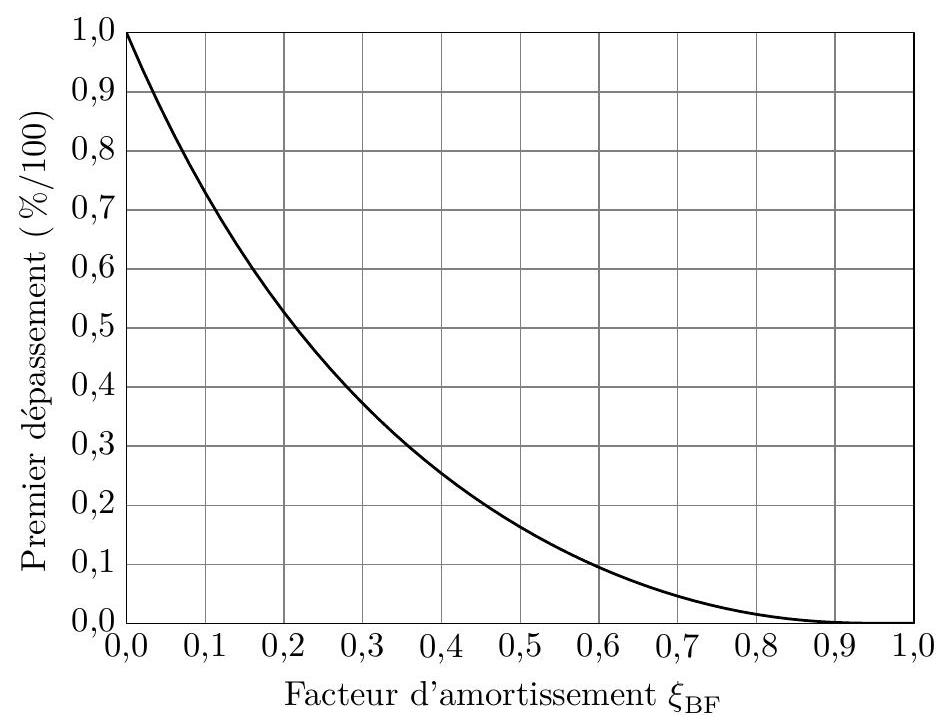
\includegraphics[width=.7\textwidth]{2025_07_06_ec63d2f3afc18cdeeb83g-07}
%Figure 9 
\caption{\label{ccs_mp_2022_fig_09}Abaque du premier dépassement}
\end{figure}
\fi


%III.B - 
\subsection{Introduction d'une correction \label{ccs_mp_2022_sec_3B}}

\begin{obj}
Pour pallier le non-respect de certaine(s) performance(s) du diagramme des exigences (figure \ref{ccs_mp_2022_fig_A}) sur le modèle $\mathrm{n}^{\circ} 1$ (figure \ref{ccs_mp_2022_fig_20}), le bureau d'études a choisi de mettre en place un correcteur dans la chaine directe, ou chaine d'action. L'objectif est de valider le choix du correcteur ainsi que son dimensionnement.
\end{obj}

%III.B.1) 
\subsubsection{Réglage d'un correcteur proportionnel vis-à-vis du critère de précision \label{ccs_mp_2022_sec_3B1}}

%Q 21. 
\question{\label{ccs_mp_2022_sec_q_21}À partir de l'expression de $\varepsilon_{a}$ déterminée à la question 19 montrer qu'un correcteur proportionnel de gain pur $K_{\text {corr.gain.pur }}$ placé dans la chaine directe, ou chaine d'action, permet d'améliorer l'erreur relative observée à la question 20.}
\ifprof
\begin{corrige}

On a $\varepsilon_\text{acc} =  \dfrac{0.3 g}{1+K_\text{BO}} $, donc si on ajoute un correcteur de type gain pur, l'erreur d'accélération deviendra :

$$\varepsilon_\text{acc} =  \dfrac{0.3 g}{1+ K_\text{corr. gain pur} \times K_\text{BO} } $$

 L'objectif étant de diminuer cette erreur, on voit que ce gain pur devra donc être supérieur à $1$. Ceci améliorera alors l'erreur relative observée à la question \ref{ccs_mp_2022_sec_q_20}.

\end{corrige}
\else
\fi


%Q 22. 
\question{\label{ccs_mp_2022_sec_q_22}Déterminer la valeur de $K_{\text {corr.gain.pur }}$ permettant d'atteindre l'exigence Id $=1.1 .1 .2 .1$.}
\ifprof
\begin{corrige}
On cherche à avoir $\varepsilon_\text{relatif} < 10\%$, d'où d'après la question \ref{ccs_mp_2022_sec_q_20} et \ref{ccs_mp_2022_sec_q_21} :
$ \varepsilon_\text{relatif} = \dfrac{1}{1 + K_\text{corr. gain pur} \times K_\text{BO}} < 0.1$
et $  1 + K_\text{corr. gain pur} \times K_\text{BO}  > \dfrac{1}{0.1} = 10$. Enfin 
$ K_\text{corr. gain pur} > \dfrac{9}{K_\text{BO}}$

A.N. : $ K_\text{corr. gain pur} > \dfrac{9}{8.4\times 10^{-3}} = 1071.4$.\end{corrige}
\else
\fi



%III.B.2) 
\subsubsection{Réglage d'un correcteur proportionnel vis-à-vis du critère de dépassement \label{ccs_mp_2022_sec_3B2}}
%Q 23. 
\question{\label{ccs_mp_2022_sec_q_23}À partir de l'expression de $\xi_{\mathrm{BF}}$ déterminée à la question \label{ccs_mp_2022_sec_q_17}, montrer qu'un correcteur proportionnel de gain pur $K_{\text {corr.gain.pur }}$ placé dans la chaine directe, ou chaine d'action, a une influence sur le dépassement observé à la question \label{ccs_mp_2022_sec_q_18}. Préciser alors le sens de variation du dépassement en fonction du gain $K_{\text {corr.gain.pur }}$.}
\ifprof
\begin{corrige}
On avait en question 18 : $\xi_\text{BF} = \dfrac{\xi_\text{BO}}{\sqrt{1 + K_\text{BO}}}$, en ajoutant un correcteur proportionnel de gain pur, le coefficient d'amortissement devient :
$ \xi_\text{BF} = \dfrac{\xi_\text{BO}}{\sqrt{1 + K_\text{corr. gain pur} \times K_\text{BO}}}$.

On remarque que plus le $K_\text{corr. gain pur}$ augmente (lorsqu'il est supérieur à $1$), plus le facteur d'amortissement diminue, ce qui implique que le dépassement sera plus important (d'après la \textsc{Figure} \ref{fig:sled9}).
\end{corrige}
\else
\fi


%Q 24. 
\question{\label{ccs_mp_2022_sec_q_24}Vérifier si l'exigence Id $=1.1 .1 .1 .2$ est respectée avec la valeur de $K_{\text {corr.gain.pur }}$ déterminée à la question \label{ccs_mp_2022_sec_q_22}.}
\ifprof
\begin{corrige}
$ \xi_\text{BF} = \dfrac{\xi_\text{BO}}{\sqrt{1 + K_\text{corr. gain pur} \times K_\text{BO}}} $
A.N. : $ \xi_\text{BF} = \dfrac{0.5}{\sqrt{1 + 476.2 \times 8.4 \times 10^{-3}}} \simeq  0.13 $.

\`A l'aide de la \textsc{Figure} \ref{fig:sled9}, on obtient un premier dépassement d'environ $0.62$, soit $62\%$.

L'exigence \texttt{Id = 1.1.1.1.2} (dépassement inférieur à $20\%$) n'est donc toujours pas respectée.

\end{corrige}
\else
\fi


%III.B.3) 
\subsubsection{Choix et réglage d'un correcteur proportionnel-intégral \label{ccs_mp_2022_sec_3B3}}
Le correcteur choisi par les ingénieurs du bureau d'études est un correcteur proportionnel-intégral, noté PI, de la forme

$$
C(p)=K_{\text {corr }}\left(\frac{1+T_{\text {corr }} p}{T_{\text {corr }} p}\right)=K_{\text {corr }}\left(1+\frac{1}{T_{\text {corr }} p}\right)=K_{\text {corr }}\left(1+\frac{\omega_{\text {corr }}}{p}\right) .
$$

%Q 25. 

\question{\label{ccs_mp_2022_sec_q_25}À l'aide des sections \ref{ccs_mp_2022_sec_3B1} et \ref{ccs_mp_2022_sec_3B2}, indiquer en quoi l'utilisation d'un correcteur proportionnel n'est pas suffisante dans le cas du Sled. Justifier le choix d'un correcteur proportionnel-intégral.}
\ifprof
\begin{corrige}
On a vu en section 3.2.1 qu'avec un correcteur proportionnel permettait de respecter l'exigence \texttt{Id = 1.1.1.2.1} concernant l'écart relatif. Mais en section 3.2.2 on s'est aperçu que le critère de dépassement (exigence \texttt{Id = 1.1.1.1.2}) ne peut être respecté (car il faudrait diminuer $K_\text{corr. gain pur}$ pour diminuer le dépassement, mais cela impliquerait que nous perdions le respect de l'exigence de précision sur l'écart relatif).\\

Un correcteur proportionnel-intégral permet d'augmenter la classe de la FTBO et donc d'avoir $\varepsilon_\text{relatif} = 0$ et cela indépendamment de la valeur de $K_\text{corr. gain pur}$. Ainsi on peut régler $K_\text{corr. gain pur}$ afin de respecter l'exigence de dépassement \texttt{Id = 1.1.1.1.2}.
\end{corrige}
\else
\fi



%Q 26. 
\question{\label{ccs_mp_2022_sec_q_26}Tracer sur la copie le diagramme asymptotique de la phase du diagramme de Bode théorique du correcteur proportionnel-intégral. Préciser ses caractéristiques principales. Compléter le diagramme asymptotique de la phase avec l'allure du diagramme réel de phase du correcteur.}
\ifprof
\begin{corrige}
La phase du correcteur s'écrit :
$\varphi = \text{arg}(K_\text{corr}) + \text{arg}\left(\dfrac{1 + j T_\text{corr} \omega}{j T_\text{corr} \omega}\right)$ $= 0 + \text{arctan}\left( T_\text{corr} \omega\right) - \text{arg}\left(j T_\text{corr} \omega\right)$
$= -90 +\text{arctan}\left( T_\text{corr} \omega\right)$


On obtient alors le diagramme de Bode suivant pour la phase :
%\begin{figure}[h!]
%\begin{tikzpicture}
%\begin{semilogxaxis}[domain=10^-1:10^5,  samples=200,  grid=both,  no markers, enlarge x limits=false, enlarge y limits=false,
%            ylabel = Phase [$\degres$\text{]},
%            xlabel = $\omega$ [rad/s\text{]},
%             width=.95\textwidth,
%             height=.5\textwidth,
%             ymin=-97, ymax=10.5,
%             ytick={0,-22,-45,-67,-90}]
%\foreach \K in {3} \foreach \tau in {0.02} {
%	\plot[blue,smooth,ultra thick, declare function={phase(\p,\a,\b)=-90+atan(\b*\p);}] 
%	(\x, {phase(\x,\K,\tau)});
%	\addplot [green, ultra thick, dashed] coordinates {(10^-1, -90) (1/\tau, -90) (1/\tau, 0) (10^5, 0)};
%	\addplot [green, thick, opacity=0] coordinates {(1/\tau, -90) (1/\tau,-45)} node[midway, anchor=north, inner sep=5, sloped, opacity=1] {\color{black}$\omega_\text{cassure} = 1/T_\text{corr}$} ;
%	\addplot [black, ultra thick, ->, >=latex] coordinates {(10/\tau, -5.7) (10/\tau,0)} node[midway, anchor=south, inner sep=5, sloped] {\color{black}$5.7\degres$} ;
%}
%\end{semilogxaxis}
%\end{tikzpicture}
%\end{figure}

\end{corrige}
\else
\fi

\ifprof
\else
Dans un premier temps, le bureau d'études souhaite régler le correcteur proportionnel-intégral afin que le modèle $\mathrm{n}^{\circ} 1$ corrigé puisse atteindre les performances de stabilité définies dans le diagramme des exigences (figure \ref{ccs_mp_2022_fig_A}). Pour cela, il utilise un programme codé en Python (figure \ref{ccs_mp_2022_fig_10}).
\begin{figure}
\centering
\begin{lstlisting}
import numpy as np

def H_BO_nc(Omega):
    # Définition de la fonction de transfert en boucle ouverte non corrigée
    K_BO = 8.4e-3 # gain en boucle ouverte non corrigée
    omegaO_BO = 71 # pulsation propre en boucle ouverte non corrigée
    Xi_BO = 0.5 # facteur d'amortissement en boucle ouverte non corrigée
    u = Omega/omegaO_BO # pulsation réduite
    FTBO_nc = K_BO/(1 + 2*Xi_BO*(1j*u) - u**2)
    return FTBO_nc
    
def reglage_PI(H_BO_nc,M_phi):
    # Détermination des paramètres du correcteur P.I. à l'aide de deux paramètres :
    # H_BO_nc : Fonction de transfert en BO du système non corrigé
    # M_phi : Marge de phase souhaitée après réglage du correcteur
    epsilon=0.5
    pas = 0.001
    Omega= 10**np.arange(0,3+pas,pas) # Pulsation de 10^0 à 10^3 en rad.s-1
    GdB_BO_nc = 20*np.log10(np.absolute(H_BO_nc(Omega))) # Gain en dB de la fonction
            # en BO non corrigée
    Phi_BO_nc = np.angle(H_BO_nc(Omega),'deg') # Phase en * de la fonction
            # en BO non corrigée
    Phi_recherchée_avant_correction= M_phi - 180 + 5.7
    i=0
    while i<len(Phi_BO_nc) and abs(Phi_BO_nc[i]-Phi_recherchée_avant_correction)>epsilon:
        i=i+1
    if i!=len(Phi_BO_nc):
        Omega_corr=Omega[i]/10 # Calcul de la pulsation de cassure du correcteur
        T_corr=1/Omega_corr # Calcul de la constante de temps du correcteur
        K_corr=10**(-GdB_BO_nc[i]/20)# Calcul du gain du correcteur
        return K_corr,T_corr
\end{lstlisting}

%Figure 10 
\caption{\label{ccs_mp_2022_fig_10}Code python de détermination du réglage du correcteur PI}
\end{figure}

\section*{Notations}
\begin{itemize}
  \item $\Phi\left(H_{\mathrm{BOnc}}\left(\omega_{c 0 \mathrm{~dB}}\right)\right)$ la phase de la boucle ouverte non corrigée à la pulsation de coupure à 0 dB .
  \item $\Phi\left(H_{\mathrm{BO}}\left(\omega_{c 0 \mathrm{~dB}}\right)\right)$ la phase souhaitée de la boucle ouverte corrigée à la pulsation de coupure à 0 dB .
  \item $M P$ la marge de phase souhaitée après correction.
\end{itemize}
\fi


%Q 27. 
\question{\label{ccs_mp_2022_sec_q_27}
Exprimer $\Phi\left(H_{\mathrm{BO}}\left(\omega_{c} 0 \mathrm{~dB}\right)\right)$ en fonction de $M P$.}
\ifprof
\begin{corrige}
$\Phi(H_\text{BO}(\omega_{c \text{0 dB}})) = -180\degres + M P$
\end{corrige}
\else
\fi

%Q 28. 
\question{\label{ccs_mp_2022_sec_q_28}Exprimer $\Phi\left(H_{\mathrm{BO}}\left(\omega_{c} 0 \mathrm{~dB}\right)\right)$ en fonction de $\Phi\left(H_{\mathrm{BO} \mathrm{nc}}\left(\omega_{c} 0 \mathrm{~dB}\right)\right)$, de $T_{\text {corr }}$ et de $\omega_{c} 0 \mathrm{~dB}$.}
\ifprof
\begin{corrige}
$\Phi(H_\text{BO}(\omega_{c \text{0 dB}})) = \Phi(H_\text{BO nc}(\omega_{c \text{0 dB}})) - 90\degres + \text{arctan}(T_\text{corr} \omega_{c \text{0 dB}})$
\end{corrige}
\else
\fi

%Q 29. 
\question{\label{ccs_mp_2022_sec_q_29}En déduire l'expression de $\Phi\left(H_{\mathrm{BO} \mathrm{nc}}\left(\omega_{c 0 \mathrm{~dB}}\right)\right)$ en fonction de $M P$, de $T_{\text {corr }}$ et de $\omega_{c 0 \mathrm{~dB}}$.}
\ifprof
\begin{corrige}
$\Phi(H_\text{BO nc}(\omega_{c \text{0 dB}})) = -90\degres + M P - \text{arctan}(T_\text{corr} \omega_{c \text{0 dB}})$.
\end{corrige}
\else
\fi

%Q 30. 
\question{\label{ccs_mp_2022_sec_q_30}Préciser comment est déterminée la pulsation de cassure du correcteur dans la méthode décrite dans le code Python de la figure \ref{ccs_mp_2022_fig_10} (ligne 26).}
\ifprof
\begin{corrige}
La pulsation de cassure du correcteur est choisi à une décade de la pulsation de coupure à $0$ dB de la fonction de transfert non corrigée. Cela implique un déphasage au niveau de la pulsation de coupure à $0$ dB de $5.7\degres$, ce qui a été pris en compte ligne 21.
\end{corrige}
\else
\fi


%Q 31. 
\question{\label{ccs_mp_2022_sec_q_31}À l'aide de l'étude précédente menée sur la correction retrouver la valeur $5,7^{\circ}$ utilisée ligne 21 dans la méthode décrite dans le code Python de la figure \ref{ccs_mp_2022_fig_10}.}
\ifprof
\begin{corrige}
En se plaçant à une décade de la pulsation de cassure du correcteur (qui est la phase de coupure à $0$ dB de la fonction de transfert non corrigée), on obtient une phase de :
$ \phi = -90 + \text{arctan}\left({T_\text{corr}} \times \dfrac{10}{{T_\text{corr}}}\right) = -90 + \text{arctan}(10) = -90 + 84.29 = -5.69\degres$.
\end{corrige}
\else
\fi

%Q 32. 
\question{\label{ccs_mp_2022_sec_q_32}Représenter cette valeur sur le tracé du diagramme de Bode de la phase du correcteur PI (question 26) et indiquer à quoi correspond cette valeur.}
\ifprof
\begin{corrige}
Cette valeur correspond au déphasage induit par l'ajout d'un correcteur dont la pulsation de cassure est située à une décade avant la pulsation de coupure à $0$ dB de la fonction de transfert non corrigée. Pour régler la marge de phase d'une fonction de transfert avec un correcteur PI par la méthode du décalage à une décade, il faut prendre en compte et régler une marge de phase de :
$M P = M P_\text{voulue} + 5.7\degres$.

Ce qui permet d'anticiper le déphasage du correcteur PI.
\end{corrige}
\else
\fi

\ifprof
\else
En utilisant la méthode de réglage du correcteur décrite dans le code Python (figure \ref{ccs_mp_2022_fig_10}), les paramètres du correcteur ont été déterminés. Les ingénieurs ont retenu les valeurs $K_{\text {corr }}=354$ et $T_{\text {corr }}=1 / 15 \mathrm{~s}=0,066 \mathrm{~s}$. La figure \ref{ccs_mp_2022_fig_11} représente le diagramme de Bode de la boucle ouverte de l'asservissement en vitesse du modèle $n^{\circ} 1$ ainsi corrigé.
\fi

%III.B.4) 
\subsubsection{Validation des exigences \label{ccs_mp_2022_sec_3B4}}
La réponse temporelle en accélération, du modèle $n^{\circ} 1$ corrigé, en réponse à la consigne d'accélération définie figure \ref{ccs_mp_2022_fig_04} est donnée sur la figure \ref{ccs_mp_2022_fig_12}.

%Q 33. 
\question{\label{ccs_mp_2022_sec_q_33}Évaluer graphiquement la marge de phase du système corrigé et conclure au regard de l'exigence Id = 1.1.1.1.1.}
\ifprof
\begin{corrige}
On lit graphiquement une marge de phase d'environ :$ M P = 42\degres > 30\degres \qquad \text{exigence \texttt{Id : 1.1.1.1.1}}$.

Ce qui respecte l'exigence \texttt{Id : 1.1.1.1.1}.
\end{corrige}
\else
\fi

%Q 34. 
\question{\label{ccs_mp_2022_sec_q_34}Évaluer le premier dépassement suite à l'échelon de consigne de $0,3 g$ et conclure au regard de l'exigence $\mathrm{Id}=1.1 .1 .1 .2$.}
\ifprof
\begin{corrige}
Le premier dépassement que l'on peut observer en \textsc{Figure} \ref{fig:sled12} est de :

$$ D_\% = \dfrac{3.6 - 3}{3} \times 100 = 0.2 \times 100 = 20\%$$

En ayant pris $3.6$ m.s$^{-2}$, nous avons surestimé la mesure, on peut donc valider l'exigence \texttt{Id : 1.1.1.1.2} qui impose un dépassement inférieur à $20\%$.
\end{corrige}
\else
\fi

%Q 35. 
\question{\label{ccs_mp_2022_sec_q_35}Conclure, en justifiant, au regard de l'exigence $\mathrm{Id}=1.1 .1 .2 .1$.}
\ifprof
\begin{corrige}
La précision indicielle est de :
$ \text{précision} = \dfrac{|0.3\times g - 3.0|}{0.3 \times g} = \left|1 - \dfrac{3.0}{0.3 \times g} \right| = \left|1 - \dfrac{10}{g}\right|$.

A.N. : $ \text{précision} = \left|1 -\dfrac{10}{9.81}\right| = 0.019 = 1.9\% < 10\% \qquad \text{exigence \texttt{Id : 1.1.1.2.1}}$.

On ne peut pas valider toutes les exigences avec les études réalisées jusqu'ici, mais les exigences \texttt{Id : 1.1.1.1.1}, \texttt{Id : 1.1.1.1.2} et \texttt{Id : 1.1.1.2.1} sont validées avec un correcteur PI réglé à une décade.
\end{corrige}
\else
\fi


\ifprof
\else
\begin{figure}[!h]
\centering
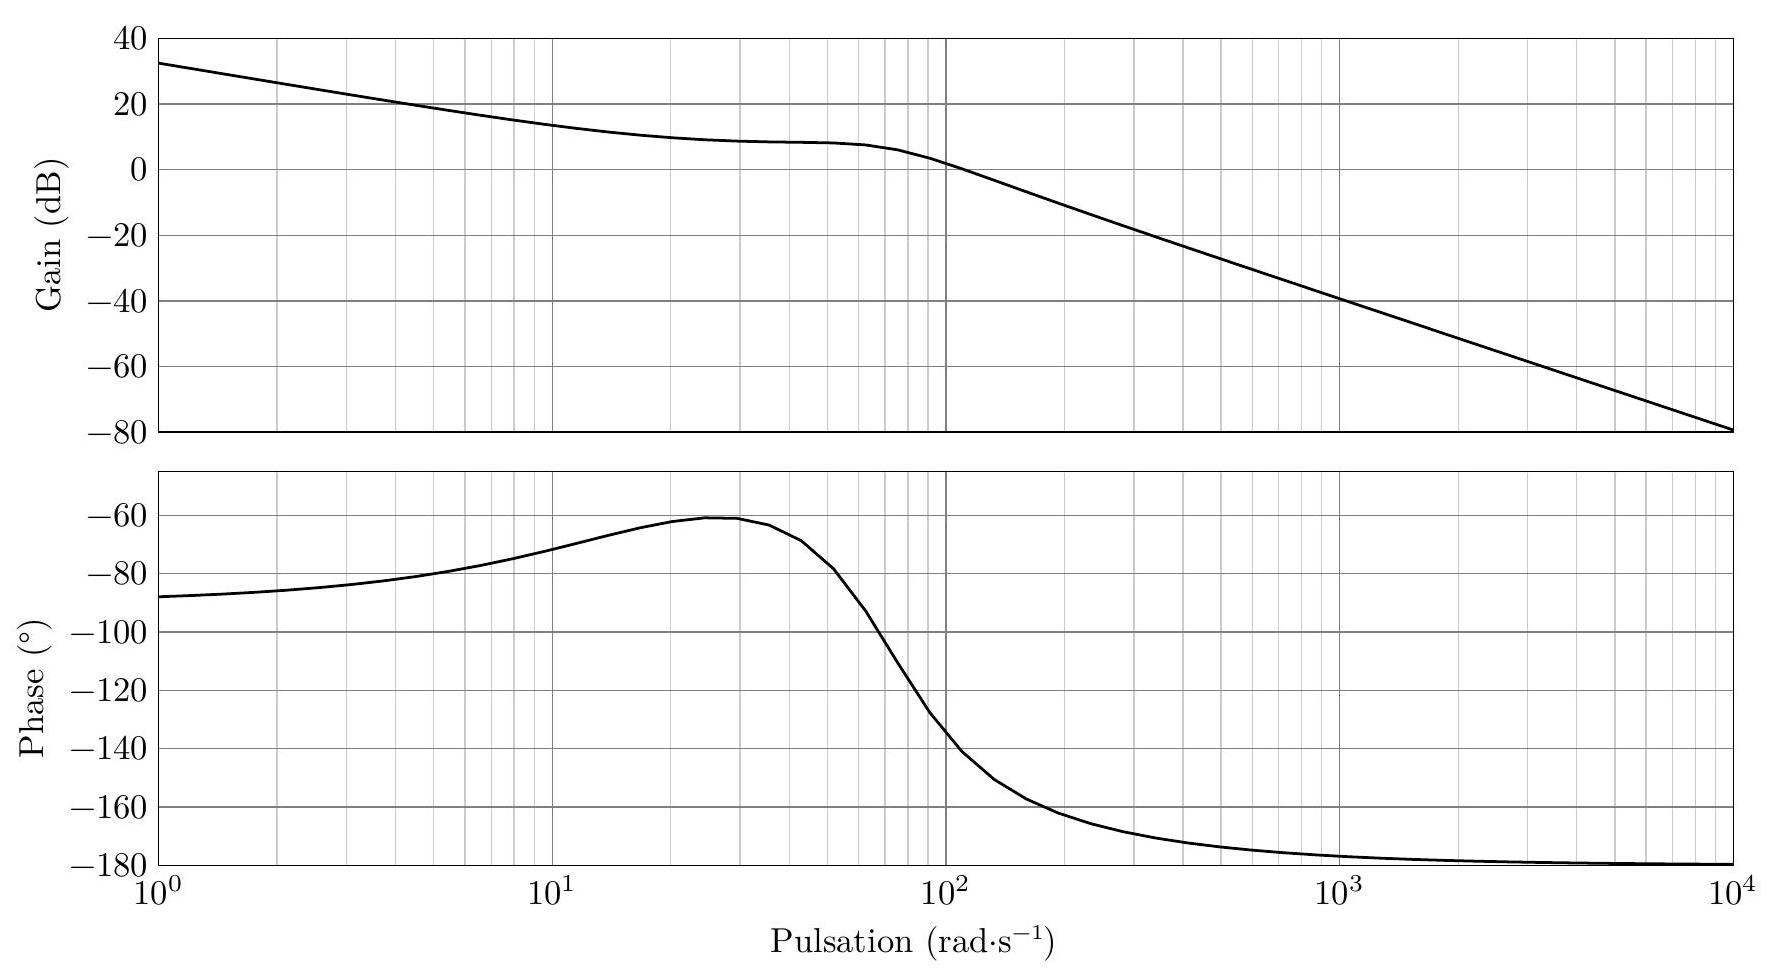
\includegraphics[width=\textwidth]{2025_07_06_ec63d2f3afc18cdeeb83g-09}

%Figure 11 
\caption{\label{ccs_mp_2022_fig_11}Diagramme de Bode de la boucle ouverte de l'asservissement en vitesse avec correction}
\end{figure}

\begin{figure}[!h]
\centering
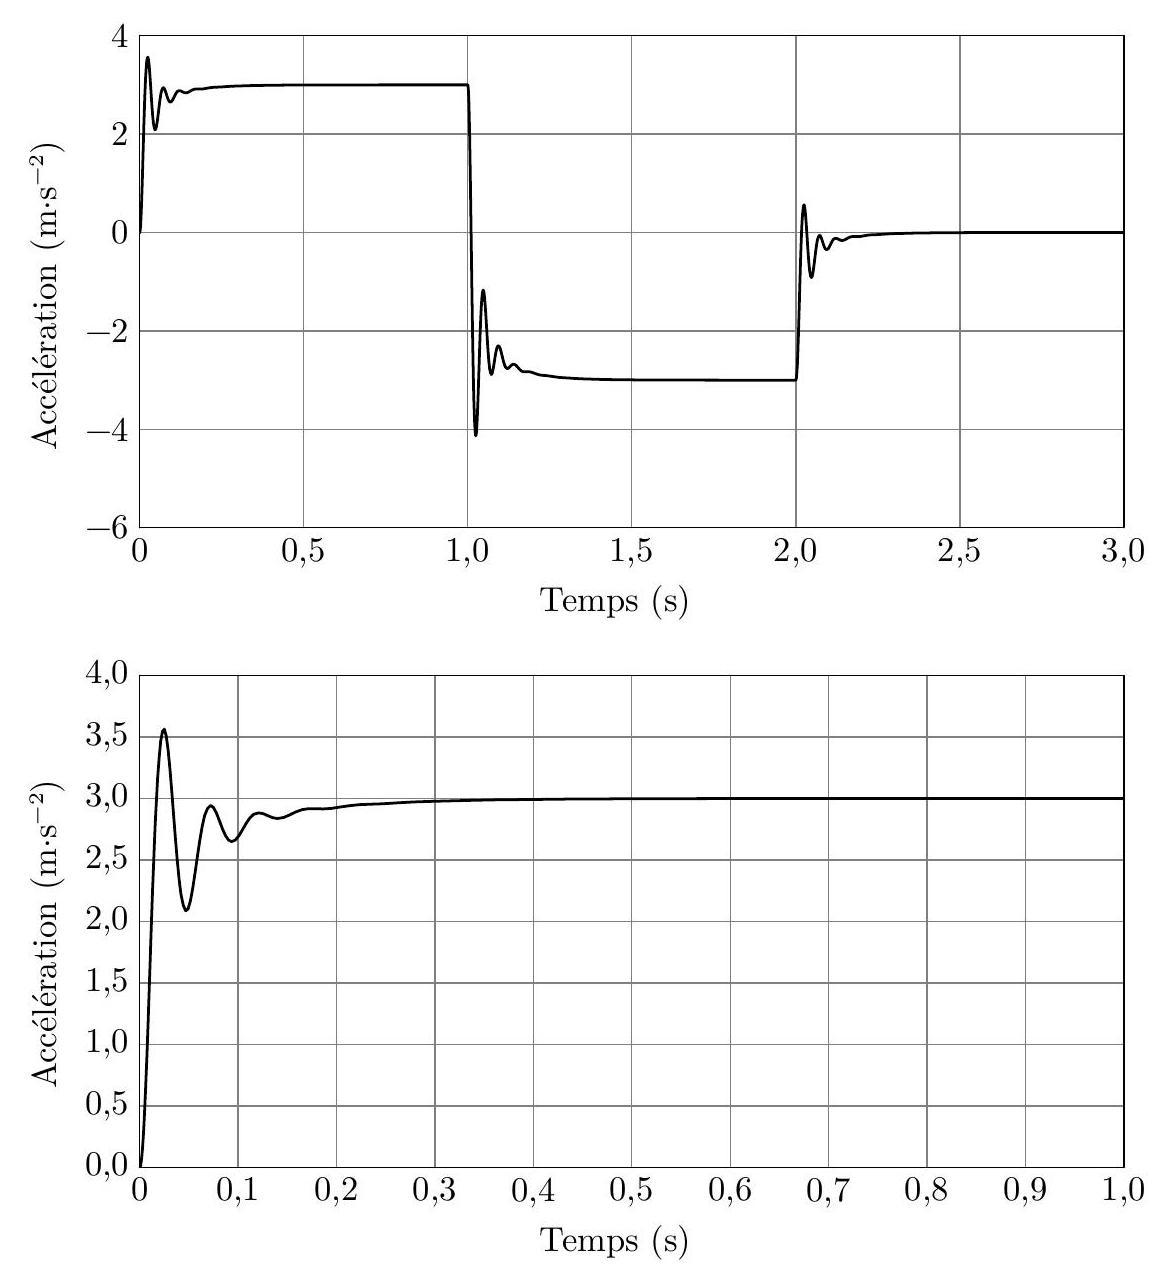
\includegraphics[width=\textwidth]{2025_07_06_ec63d2f3afc18cdeeb83g-09(1)}

%Figure 12 
\caption{\label{ccs_mp_2022_fig_12}Réponse temporelle en accélération du système corrigé (au-dessus) et zoom (en dessous) sur l'échelon de consigne $0,3 g$}
\end{figure}

Les ingénieurs du bureau d'études décident d'arrêter en l'état la modélisation du Sled $0,3 g$ qui a permis de définir une première structure de commande. Ils souhaitent à présent s'investir dans la réalisation d'un Sled et mener des expérimentations.
\fi
